% Chapter 1

\chapter{Introduction to Wireless Sensor Networks} % Main chapter title
\label{Chapter1} % To reference to this chapter elsewhere, use \ref{Chapter1} 
\lhead{Chapter 1. \emph{Sound nomenclature}} % This is for the header on each page - perhaps a shortened title
%\textsf{\textsl{Written by Bjorn Deraeve}}
%----------------------------------------------------------------------------------------
\begin{center}
{\textsl{What if: }}
\begin{large}
\textbf{Ubiquitous Computing \& Networking} + \textbf{Sensing \& Control} ?
\end{large}
\end{center}


\section{Introduction}
The ENIAC, the first electronic computer designed by the American scientists J. Presper Eckert and John W. Mauchly, Turing-complete,  pioneering in 1946 and designed to calculate artillery firing tables. A wireless sensor network node, over 50 years later and 10 million times less the size of the ENIAC, still Turing-complete, and still military roots.\\
The origins of the research to Wireless Sensor Networks (WSNs) can be traced back to DARPA\footnote{Defense Advanced Research Projects Agency (DARPA), is an American agency responsible for developing military technologies. DARPA has fund the research in many technologies which have had major effect on the world, including ARPANET, the first wide-area packet switching network (ancestor of the Internet and Douglas Engelbart's precursors to the GUI.}, which sponsored a workshop at Carnegie Mellon University in 1978, identifying the technology components for a DSN. But at the time the technology was not quite ready. Sensors could take up the size of a shoe box and up, limiting the number of potential applications. The earliest DSNs were also not very tightly associated with wireless communication.\\
In 1998 a new wave of research in WSNs started. Again DARPA acted as pioneer by launching the initiative research program 'SensIT', which added new capabilities to the current sensor network such as ad hoc networking, dynamic querying and tasking, reprogramming and multi-tasking. At the same time IEEE noticed the high capabilities and low expenses of WSNs and defined the IEEE 802.15.4 standard for low power consumption, low data rate wireless PANs. for 868MHz, 915MHz and 2.4GHz radios. Finally, in 2002, the ZigBee Alliance was established and published the ZigBee standard, based on IEEE 802.15.4. The standard adds a suite of high level communication protocols for WSNs such as device coordination, network topologies and interoperability with other wireless products.\\
Currently, WSNs are seen as one of the most prospective technologies of the 21st century (21 Ideas for the 21st Century, 1999). China for example, has involved WSNs in their national strategic research programmes (Program 973). The project follows an application-driven methodology and aims to issues identified with the real-world critical problems facing Chinese society. Over the years the program has funded areas such as agriculture, health, resources, energy, population and materials and brought significant benefits to China's sustainable economic and social development.
%----------------------------------------------------------------------------------------
\section{Wireless is everywhere}
\subsection{Definition of Wireless Sensor Network}
\emph{A Wireless Sensor Network (WSN) consists of spatially distributed autonomous sensors connected via a (wireless) communications infrastructure to cooperatively monitor, record and store physical or
environmental conditions, such as temperature, sound, vibration, pressure, motion or pollutants} (Sebastian B\"uttrich)
%---------------------------------
\subsection{Internet of Things}
The Internet of Things is a term that was first used by Kevin Ashton\footnote{Kevin Ashton co-founded the Auto-ID Center at the  Massachusetts Institute of Technology (MIT). The Center is a research group in networked RFID and newly emerging sensing technologies. The main goal was the development of the Electronic Product Code (EPC), a global RFID-based item identification system intended to replace the UPC bar code} in 1999 and answers the question introducing this chapter. It refers to uniquely identifiable objects (things) and their virtual representations in an Internet-like structure. It is a vision of a network of Internet-enabled objects, together with web services which interact with these objects. If all objects in the world would be equipped with minuscule identifying devices this could transform our daily lives. By embedding computational capabilities in all kinds of objects, including living beings, it will be possible to provide qualitative and quantitative shift in several sectors: logistics, domotics, healthcare, entertainment, and so on.\\
WSNs can provide a virtual layer where the information about the physical world can be accessed by any computational system. As a result, WSNs are one of the most important elements for realizing the vision of the Internet of Things paradigm. On May 2nd, 2012, Libelium\footnote{The manufacturer of the Hardware we used. See chapter \ref{Chapter3} for more information.} published a list of 50 cutting edge \emph{Internet of Things} applications . According to Libelium, by 2020, more then 50 billion devices will be connected to the Internet.\\
%---------------------------------
\subsection{Third wave of wireless}
The IoT can also be considered as the third wireless wave. Following cellular technology and WiFi, today wireless technology also includes the world of sense and control technology to bridge the gap between the virtual electronic world and our human physical world. This wave is not focussed on enhancing human communication. Instead it allows sensors to interact with actuators, creating a more dynamic world and avoiding costly human labour. Finally, as the title of this section suggests, WSNs offer the ability to observe the previously unobservable.
%---------------------------------------------------------------------------------------- 
\section{Wireless Standards and Technology}
\subsection{Standards enable growth: ZigBee}
Not only do standards allow devices from different vendors to interoperate, they also provide OEMs and integrators the flexibility of second sourcing. The ZigBee Alliance is an independent standardization organization which is driven by a large group of OEM companies and has definitely had a large impact on the rapid development of WSNs.\\
\begin{figure}[htbp]
\centering
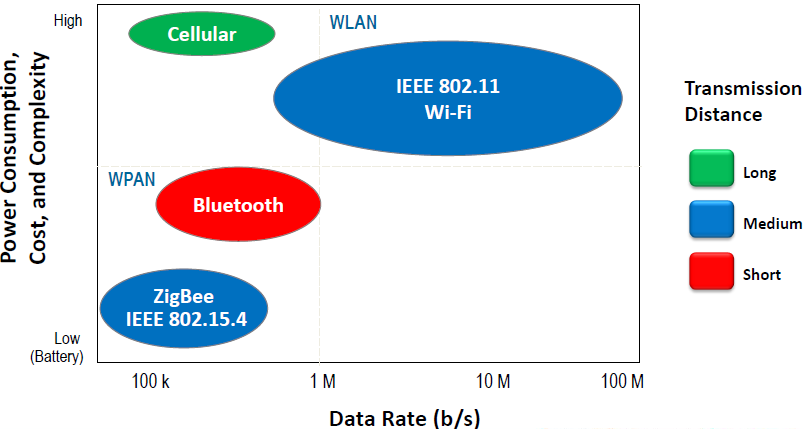
\includegraphics[height=6cm]{zigbeeRange}
\rule{30em}{0.5pt}
\caption{Comparing the ZigBee standard with Cellular, Bluetooth and WiFi}
\label{fig:stand}
\end{figure} \\
Figure \ref{fig:stand} indicates the most critical properties of the ZigBee standard. Some rules-of-thumb are:
\begin{itemize}
\item The higher the frequency, the higher the data rate and power consumption
\item The lower the frequency, the further the reach
\item All radio waves show strong absorption in water and metal 
\end{itemize}
Table \ref{tab:range} shows the typical power consumption, throughput, range and application examples of each technology:
\begin{table}[!ht]
\begin{center}
\begin{tabular}{cc|c|c|c|l}
\cline{2-5}
 & \multicolumn{1}{ |c| }{\textbf{Battery Life}} & \textbf{Data Rate} & \multicolumn{1}{|c|}{\textbf{Range}} & \textbf{Application Examples}\\ \cline{1-5}
%\multicolumn{1}{ |c| }{Sleep duration} & High Performance & Power Saver & High Performance & Power Saver    \\ \cline{1-5}
\multicolumn{1}{ |c| }{\textbf{ZigBee}} & 1-4 years & 20 to 250Kbps & 100 m & Wireless Sensor Networks    \\ %\cline{1-5}
\hline
\multicolumn{1}{ |c| }{\textbf{Bluetooth}} & 1-2 weeks & 1 to 3 Mbps & 10 m & Wireless Headset   \\ %\cline{1-5}
\hline
\multicolumn{1}{ |c| }{\textbf{IEEE 802.11g}} & 1-2 days & 6 to 54Mbps & 30 m & Wireless Internet Connection   \\ %\cline{1-5}
\hline
\end{tabular}
\caption{Comparing the ZigBee standard with Cellular, Bluetooth and WiFi}
\label{tab:range}
\end{center}
\end{table}\\
%---------------------------------
\subsection{Sensor nodes}
Sense
Compute
Store
Communicate
%---------------------------------
\subsection{Fundamental Challenges in WSNs}
The biggest challenge WSNs encounter is without a doubt power consumption. Power! Power! Power! The next section will briefly introduce the general concepts and in section \ref{powerSect} the power consumption of the WSN we developed will be analyzed thoroughly. Other challenges often fall back to this limited amount of available energy, security for example.\\
There are dozens of other basic challenges for WSNs. Unattended operation and environmental influence makes a mote prone to failure. Mobility can cause topology changes. WSNs can use over more than 100 nodes, this leads to scalability issues and synchronization issues. There must also be a form of synchronization with sleeping nodes. Network responsiveness and robustness (this will be discussed more in section \ref{pow}.  Not to forget making sense out of sensors.\\
%---------------------------------
\subsection{Power considerations}
\begin{figure}[htbp]
\centering
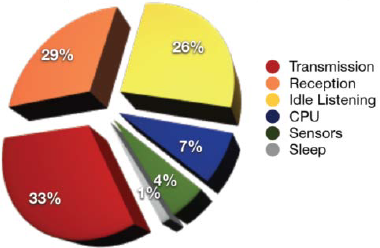
\includegraphics[height=6cm]{typicalCons}
\rule{30em}{0.5pt}
\caption{Typical power consumption of a node}
\label{fig:typicalCons}
\end{figure} 
\begin{figure}[htbp]
\centering
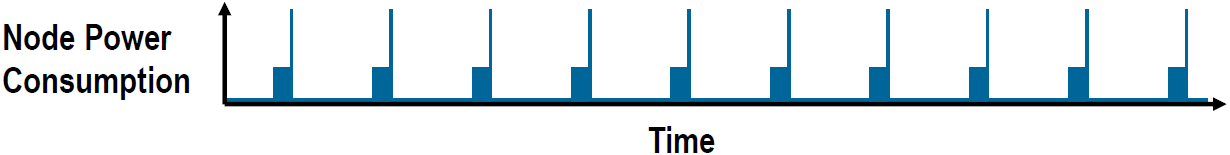
\includegraphics[height=6cm]{powerCons}
\rule{30em}{0.5pt}
\caption{Typical power consumption of a node}
\label{fig:typicalCons}
\end{figure} 

%---------------------------------
\subsection{Network topologies}
%---------------------------------
\subsection{Security}

%----------------------------------------------------------------------------------------
\section{Benefits of Wireless Measurements}
Wireless Sensor Networks provide benefits in roughly three categories:
\begin{enumerate}
\item Reduce costs
\begin{itemize}
\item Installation costs and time
\item Maintenance costs
\end{itemize}
\item Increase efficiency
\begin{itemize}
\item Optimize measurement processes
\item Access data everywhere and every time
\item Decrease downtime
\end{itemize}
\item Monitor anywhere
\begin{itemize}
\item Overcoming power or infrastructure limitations
\item Solve new and previously challenging applications
\end{itemize}
\end{enumerate}
\section{WSNs: Innovative ways of interacting with the world}
pdf intro to sensornets


%----------------------------------------------------------------------------------------


